\renewcommand{\thetable}{S\arabic{table}}
\setcounter{figure}{0}
\renewcommand{\thefigure}{S\arabic{figure}}

\section{Supplementary Materials}

\begin{sansmath}
\py{pytex_fig('scripts/msc_violin.py',
        conf='article/1col.conf',
        label='mscv',
        caption='
                \\textbf{The Generic Masked workflow does not introduce a loss of significance.}\\
                Comparison across workflows and functional contrasts.
                ',
        multicol=True,
        )}
\end{sansmath}

\py{pytex_subfigs(
	[
		{'script':'scripts/map_generic_cbv.py', 'label':'mggc', 'conf':'article/map.conf', 'options_pre':'{.48\\textwidth}',
			'caption':'
				The Generic workflow together with the CBV map shows a correct slice orientation and a coverage that is correctly bounded to the acquisition area.
				'
			,},
		{'script':'scripts/map_generic_masked_cbv.py', 'label':'mllc','conf':'article/map.conf', 'options_pre':'{.48\\textwidth}',
			'caption':'
				The Generic Masked workflow together with the CBV map shows a correct slice orientation and a coverage that is correctly bounded to the acquisition area.
				'
			,},
		{'script':'scripts/map_generic_bold.py', 'label':'mggb', 'conf':'article/map.conf', 'options_pre':'{.48\\textwidth}',
			'caption':'
				The Generic workflow together with the BOLD map, shows a correct slice orientation and coverage that is correctly bounded to the acquisition area.
				'
			,},
		{'script':'scripts/map_generic_masked_bold.py', 'label':'mllb','conf':'article/map.conf', 'options_pre':'{.48\\textwidth}',
			'caption':'
				The Generic Masked workflow together with the BOLD map, shows a correct slice orientation and coverage that is correctly bounded to the acquisition area.
				'
                        ,},
		],
	caption='
                \\textbf{The Generic Masked workflow does not induce statistic coverage misalignment nor does it induce overflow of the statistic maps into adjacent anatomical regions.}
				Four multiplanar depictions of second-level omnibus statistic maps thresholded at $\mathrm{|t|\geq2}$ are shown, corresponding to CBV and BOLD scans.
				The acquisition area is outlined by the pink square.
                ',
	label='fig:m',)}

\begin{figure*}[h!]
	\centering
	\begin{subfigure}[t]{0.48\textwidth}
		\centering
		\setlength{\fboxsep}{0pt}%
		\setlength{\fboxrule}{0.2pt}%
		\fbox{
			\includegraphics[width=\textwidth]{data/manual_overview/generic/4008_ofMcF1_cbv} 
			}
		\caption{
			SAMRI Generic workflow, depicting an undistorted functional scan intermediary;
			\vspace{1em}
			}
		\label{fig:fit_gg}
	\end{subfigure}\hfill
	\begin{subfigure}[t]{0.48\textwidth}
		\centering
		\setlength{\fboxsep}{0pt}%
		\setlength{\fboxrule}{0.2pt}%
		\fbox{
			\includegraphics[width=\textwidth]{data/manual_overview/generic/4008_ofMcF1_T2w} 
			}
		\caption{
			SAMRI Generic workflow, depicting an undistorted structural scan intermediary;
			\vspace{1em}
			}
		\label{fig:fit_gga}
	\end{subfigure}
	\begin{subfigure}[t]{0.48\textwidth}
		\centering
		\setlength{\fboxsep}{0pt}%
		\setlength{\fboxrule}{0.2pt}%
		\fbox{
			\includegraphics[width=\textwidth]{data/manual_overview/generic_masked/4008_ofMcF1_cbv}
			}
		\caption{
			SAMRI Generic Masked workflow, depicting an undistorted functional scan intermediary;
			}
		\label{fig:fit_ll}
	\end{subfigure}\hfill
	\begin{subfigure}[t]{0.48\textwidth}
		\centering
		\setlength{\fboxsep}{0pt}%
		\setlength{\fboxrule}{0.2pt}%
		\fbox{
			\includegraphics[width=\textwidth]{data/manual_overview/generic_masked/4008_ofMcF1_T2w}
			}
		\caption{
			SAMRI Generic Masked workflow, depicting an undistorted structural scan intermediary;
			}
		\label{fig:fit_lg}
	\end{subfigure}
	\caption{
		\textbf{The SAMRI Generic Masked provides a more accurate coverage of the template space.}
		Depicted are slice-by-slice inspections of the registration fit, with a spacing that is analogous to acquisition.
		}
	\label{fig:fit}
\end{figure*}

\begin{figure*}[h!]
	\centering
	\begin{subfigure}[t]{1\textwidth}
		\centering
		\setlength{\fboxsep}{0pt}%
		\setlength{\fboxrule}{0.2pt}%
		\fbox{
			\includegraphics[width=\textwidth]{data/manual_overview/generic/coherence_4008_cbv}
			}
		\caption{A slice-by-slice overview of the SAMRI Generic registration coherence across multiple sessions.}
	\end{subfigure}
\end{figure*}
\begin{figure*}[h!]\ContinuedFloat
	\begin{subfigure}[t]{1\textwidth}
		\centering
		\setlength{\fboxsep}{0pt}%
		\setlength{\fboxrule}{0.2pt}%
		\fbox{
			\includegraphics[width=\textwidth]{data/manual_overview/generic_masked/coherence_4008_cbv}
			}
		\caption{A slice-by-slice overview of the SAMRI Generic Masked registration coherence across multiple sessions.}
	\end{subfigure}
	\caption{
		\textbf{Both the SAMRI Generic and the Generic Masked workflow present a consistent mapping across sessions.}
		}
 	\label{fig:coherence}
\end{figure*}

\begin{figure*}[h!]
	\begin{subfigure}{0.75\textwidth}
		\centering
		\includedot[width=\linewidth]{data/generic_nipype}
		\vspace{-1.9em}
		\caption{
			“SAMRI Generic” workflow, based on the \textcolor{mg}{\texttt{antsRegistration}} function.
		}
		\label{fig:nwfgg}
	\end{subfigure}
	\begin{subfigure}{0.75\linewidth}
		\centering
		\includedot[width=\textwidth]{data/generic_masked_nipype}
		\vspace{-1.9em}
		\caption{
			“SAMRI Generic Masked” workflow, which is based on the \textcolor{mg}{\texttt{antsRegistration}} function.\\
		Two additional nodes provide the workflow with both the masked image and the binary mask.
			}
		\label{fig:nwfgl}
	\end{subfigure}\hfill
	\caption{
		Directed acyclic graphs visualising the two registration workflows.
		Each node name is depicted together with its corresponding package name in paranthesis.
		The “utility” indication corresponds to nodes based on Python functions specific to the workflow, distributed alongside it, and dynamically wrapped via Nipype.
		}
	\label{fig:nwfg}
\end{figure*}

%\py{pytex_tab('scripts/stim_table.py',
%                label='stim',
%                caption='Stimulation protocol, as delivered during functional scans.
%                        Stimulus event spacing and parameters are constant across scans, but the exact onset time is variable in the \SI{10}{\second} magnitude range due to scanner adjustment time variability.',
%                options_pre='[htp] \\scriptsize \\centering \\resizebox{\\columnwidth}{!}{',
%                data='data/JogB.tsv',
%                options_post='}',
%                )}

